% ----------------------------------------------------
% Firmware Submodule
% ----------------------------------------------------
\chapter{Firmware development \label{ch:firmware}}
\section{Subsystem introduction}

This subsystem deals with the development of firmware for the microcontrollers in both the camera/transmitter and receiver modules. The fundamental goals of this subsystem are to enable the camera/transmitter module to take photographs of the red-winged starlings, and to transmit this photographs to the receiver module without disturbing the birds' nests. The source code for this subsystem is available in the \href{https://github.com/rothdu/EEE4113F-Group13-2024}{project repository} on GitHub.

Section \ref{s:firmware-requirements} presents a traceability matrix with the subsystem's user requirements, interpretted functional requirements, and the corresponding ATPs. Section \ref{s:firmware-design-decisions} discusses high-level design decisions that informed the subsystem development process. Section \ref{s:firmware-design-process} details the design process and the functionality of the final implementation. Finally, section \ref{s:firmware-atps} shows the acceptance test procedures, proving that the user requirements have been adequately met.

\section{Requirement analysis} \label{s:firmware-requirements}
User requirements (UR) where determined from discussions with the red-winged starling researchers \cite{hofmeyer2024private}. The user requirements were interpretted to form functional requirements (FR) for the subsystem, and subsystem specifications (SS). These are reflected in Table \ref{tab:firmware-requirements}

\begin{table}[!ht]
    \centering
    \begin{tabularx}{\textwidth}{|p{0.13\textwidth} X|}
        
        \hline
        \textbf{UR/FR/SS} & \textbf{Description}\\ \hline
        \textit{UR1} & Triggered with movement\\
        \textit{FR1} & Image capture triggered quickly after PIR sensor reading to see the object that moved\\
        \textit{FR2} & Image capture fast enough to see object that moved\\
        \textit{SS1} & Image capture triggered on PIR sensor high\\ 
        \textit{SS2} & Image captures within 1 second of PIR trigger\\ \hline

        \textit{UR2} & Data access without disturbing nests\\
        \textit{FR3} & A wireless communication protocol must be set up to transfer camera/transmitter data to the receiver\\
        \textit{SS3} & Appropriate two-way communication protocol using WiFi chosen\\
        \textit{SS4} & Protocol transmits all images from the camera/transmitter to the receiver\\ \hline

        \textit{UR3} & Repeated photographs or video footage\\
        \textit{FR4} & Camera must capture multiple time per trigger or take video footage\\
        \textit{SS5} & Module captures a configurable number \textit{n} images each time it is triggered\\ \hline

        \textit{UR4} & Access to images in real time\\
        \textit{FR5} & Tranmission from the camera/transmitter module must be available on-demand from the receiver module\\
        \textit{SS6} & Transmission from the camera/transmitter to the receiver is triggered by a high reading from the RF linker\\ \hline

        \textit{UR5} & Data gathering over 7-week breeding season without frequent camera/transmitter battery changes\\
        \textit{FR6} & Camera/transmitter module must utilise power-saving modes where possible\\
        \textit{SS7} & Camera/transmitter module enters deep sleep mode after finishing image capture or data transmission \\ \hline

        \textit{UR6} & Configurable image quality and trigger frequency\\
        \textit{FR7} & Camera/transmitter module must include remotely updateable configuration options\\
        \textit{SS8} & Camera/transmitter module reads a configuration file in initialisation and loads the appropriate configuration values \\
        \textit{SS9} & New configuration file can be sent from receiver to camera/transmitter which is loaded on next camera/transmitter boot \\ \hline

        \textit{UR7} & Deployment of multiple camera/transmitter modules for different nests\\
        \textit{FR8} & Receiver device must handle separate image storage and configuration options for many camera/transmitter modules\\
        \textit{SS10} & Each module stores and transmits a unique device ID\\
        \textit{SS11} & Receiver module stores a separate folder for data relating to separate deployed modules\\ \hline

    \end{tabularx}
    \caption{Requirement and specification analysis for the firmware subsystem}
    \label{tab:firmware-requirements}
\end{table}



\section{High-level design decisions } \label{s:firmware-design-decisions}

This section details high-level design decisions that were made prior to any implementation and testing. These decisions determined key aspects of the development process.

\subsection{Development environment}

Both the ESP32 used for the camera/transmitter and the Raspberry Pi Pico W used for the receiver support a variety of code development environments, including their own native C/C++ frameworks, Arduino, MicroPython and CircuitPython. A summary of the support and features of the various coding frameworks is presented in Table \ref{tab:coding-env}.

\begin{table}[ht]
    \centering
    \begin{scriptsize}
    \begin{tabularx}{0.7\textwidth}{|b{0.08\textwidth}|p{0.2\textwidth}|X|X|X|}
    \hline
    \textbf{Device}                      & \textbf{Environment}        & \textbf{Library support} & \textbf{Online support/userbase} & \textbf{Abstraction level} \\ \hline
    \multirow{4}{0.08\textwidth}{ESP32}              & \color{black} \textit{C/C++ with ESP-IDF} & \color{ForestGreen} Extensive  & \color{ForestGreen} Extensive & \color{red} Low \\ \cline{2-5} 
                                         & \color{black} \textit{Arduino}            & \color{ForestGreen} Extensive  & \color{ForestGreen} Extensive & \color{ForestGreen} Moderate \\ \cline{2-5} 
                                         & \color{black} \textit{MicroPython}        & \color{red} Limited & \color{red} Minimal & \color{CadetBlue} High \\ \cline{2-5} 
                                         & \color{black} \textit{CircuitPython}      & \color{red} Limited & \color{red} Minimal  & \color{CadetBlue} High \\ \hline
    \multirow{5}{0.08\textwidth}{Raspberry Pi Pico W} & \color{black} \textit{Native C/C++ SDK}   & \color{CadetBlue} Moderate  & \color{CadetBlue} Moderate & \color{red} Low\\ \cline{2-5} 
                                         & \color{black} \textit{Official Arduino port}  & \color{CadetBlue} Moderate & \color{CadetBlue} Moderate & \color{ForestGreen} Moderate \\ \cline{2-5} 
                                         & \color{black} \textit{Community Arduino port}  & \color{ForestGreen} Extensive & \color{ForestGreen} Extensive & \color{ForestGreen} Moderate \\ \cline{2-5} 
                                         & \color{black} \textit{MicroPython}        & \color{ForestGreen} Extensive  & \color{ForestGreen} Extensive & \color{CadetBlue} High \\ \cline{2-5} 
                                         & \color{black} \textit{CircuitPython}      & \color{ForestGreen} Extensive & \color{CadetBlue} Moderate & \color{CadetBlue} High \\ \hline
    \end{tabularx}%
    \end{scriptsize}
    \caption{Summary of common coding environments for the available microcontroller}
    \label{tab:coding-env}
\end{table}

With the exception of MicroPython and CircuitPython for the ESP32, the library and online support is likely sufficient for this application. Abstraction level is thus a key consideration. Frameworks with low extraction levels are typically used in professional applications that require fine control over the device hardware. This often makes using these frameworks much more time consuming, unless you have extensive experience with the framework. On the other hand, high abstraction levels sometimes abstract away desired hardware control. A moderate abstraction level is preferred, to strike a balance between these considerations.

Arduino thus emerges as a clear choice for the ESP32. Although MicroPython and CircuitPython may provide all the functionality needed for the the Raspberry Pi Pico W, Arduino was chosen such that the entire project was coded in the same framework, thus requiring knowledge of only the one framework in the current and future iterations of the project.

The Raspbery Pi Pico W supports two Arduino ports - the "official" one, and a community maintained one. Contrary to what might be expected, the community port offers better library and online/user support, as it has been in development for longer; thus, the community port was used.

\subsection{File transfer method}

As described in Chapter , the WiFi was selected as the preffered communication method on a hardware level. Both microcontrollers also support Bluetooth, but this was largely coincidental.
%TODO: Add reference to Thiyashan's section

For data transmission over WiFi, numerous protocols exist, including encrypted and unencrypted protocols. An encrypted protocol was not necessary for this application, as the devices did not transmit sensitive data. The encryption involved inherently makes them more complex and often less efficient; as such, only unencrypted protocols were considered.

Standard unencrypted protocols include User Datagram Protocol (UDP), Tranmission Control Protocol (TCP), File Transfer Protocol (FTP) and Hypertext Transfer Protocol (HTTP). UDP and TCP are low-level protocols; using a standard higher-level prtocol such as FTP or HTTP is more appropriate unless very fine control of data transmission is needed. FTP and HTTP both operate on top of TCP. Of FTP and HTTP, HTTP is much more widely used owing to its use in the World Wide Web, and thus has better library support and documentation, thus it was chosen as the preffered option.

\subsection{Server and client location}

Communication over HTTP is based on a client-server model, where a client sends a request to a known host. It was decided that the camera/transmitter module would act as the client, while the server would be hosted on the receiver. In the current iteration of the project, either device could viably be the server or the client, given HTTP supports two-way communication. 

However, in future iterations of the project, there are particular merits to hosting the server on the receiver device. The server requires a known IP address such that the client knows where to direct it's requests. Once a client has connected to the server, the server sends it's response directly back to whatever client responded to it. The network settings of the UCT campus WiFi do not allow devices to set static IP addresses, meaning it is impossible to host the server on the campus WiFi. If the camera/transmitter acts as the client, it does not need a known IP address when connected to campus WiFi, and could connect to a remotely hosted server. To save power on the camera/transmitter module, it could also be useful to allow the module to immediately initiate connection to the server by acting as the client. 

Aditionally, hosting the server on the receiver device allows for traditional web browsers to remotely connect as a client. This could allow for applications such as updating configuration stored configuration or viewing stored images on the receiver device from a smartphone or laptop.

\subsection{Library selection}

The Arduino framework includes a wide variety of software libraries. These include "standard" libraries, which are integrated into the Arduino framework or the Arduino core for a particular device, and user-supplied libraries which are uploaded by Arduino users. In most cases, the "standard" libraries have the best support and documentation, and are known to be relatively bug-free; as such, "standard" libraries were used for all applications for which they were available.

Some specific library selections falling outside of this general principle were:

\begin{itemize}
    \item ArduinoJson cites 10\% better speed and memory efficiency than the "standard" library, and has extensive documentation available on its website.
    \item ScreenUI  is a user-implemented library for easy development of menus which display on LCD screen, which was applied to the receiver module.
    \item Reference I2C library here...
\end{itemize}

% TODO: reference the libraries I've used



\section{Submodule design} \label{s:firmware-design-process}

\subsection{High level camera/transmitter module firmware flow}

\begin{figure}[ht]
    \centering
    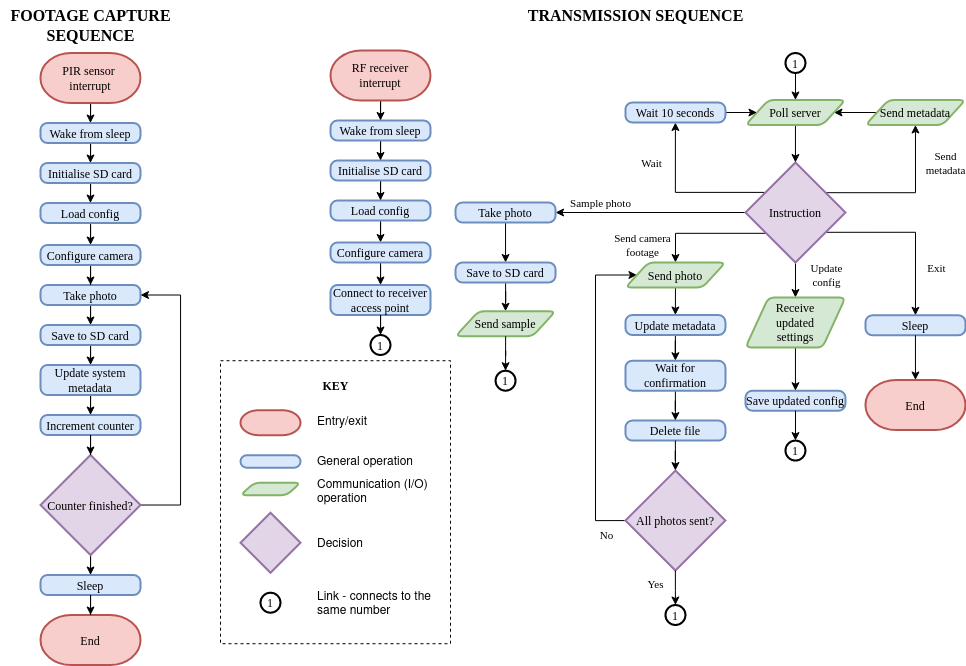
\includegraphics[width=\columnwidth]{"Images/ESP-flow.png"}
    \caption{Flowchart representing the program flow of the ESP32 Camera/Transmitter module}
    \label{fig:espflow}
\end{figure}

Figure \ref{fig:espflow} demonstrates a high-level program flow of the Camera/Transmitter module. The two sequences operate independently. The module has two primary purposes - capturing footage, and transmitting it. Footage capture is Transmission can be triggered manually from the reveiver module, with an interrupt that comes via the RF receiver. 

\subsection{HTTP server API}

The HTTP server implemented on the receiver module or a standalone computer must have available endpoints for all the applications the client wishes to utilise.

\subsection{Camera/transmitter module configuration file}

To meet the identified soft-configurability requirement, the ESP32 module will read a customiseable configuration file to determine a number of key settings. The configuration file is stored in plaintext json at "starling-cam/config/config.json" on the microSD card. If the configuration file is unavailable or unreadable, or any configuration parameters are invalid or missing, any missing parameters are loaded as defaults.

This configuration option has a number of advantages:

\begin{itemize}
    \item Storing configuration on the microSD card makes it possible to load new configuration options without needing to flash new code onto the ESP32 or access it remotely.
    \item JSON is human-readable format, making easily possible to write new configuration files.
    \item JSON is a well-supported format, and can easily be read and interpretted on the ESP32 using the ArduinoJson library % TODO \ref{arduinoJSON ref here}
\end{itemize}

\subsection{Camera sensor settings}

The user requirements specified that video or image capture was acceptable, though for the latter a number of images in quick succession would be preferable. A key limitation in this regard was the microSD card on the camera/transmitter module, which had to be formatted with the FAT32 filesystem in order for the module to interface with it. FAT32 is an older file system which only supports up to 4GB of storage. This storage limitation made still image capture more feasible, especially allowing for the possibility that images would be captured many time each day.

% TODO: Probably some test about file size and a proper analysis of photo vs video

% TODO: A proper analysis of the settings available

\subsection{Camera speed testing}


\section{Acceptance Tests \label{s:firmware-atps}}

% Things that need to be implemented:
% Receiver:

% \begin{itemize}
%     \item I2C Led display library
%     \begin{itemize}
%         \item %https://github.com/T-622/RPI-PICO-I2C-LCD/tree/main
%         \item %https://github.com/dhylands/python_lcd
%         \item %https://github.com/peterhinch/micropython-async/tree/master/v3/as_drivers/hd44780
%     \end{itemize}
%     \item Pushbutton inputs
%     \item \begin{itemize}
%         \item Seems to be fine on pi pico
%     \end{itemize}
%     \item Writing to SD card
%     \begin{itemize}
%         \item probably just the default arduino SD library
%     \end{itemize}
%     \item Web server and data reception
%     \item RFID transmitter usage
% \end{itemize}

% Camera:
% \begin{itemize}
%     \item Read/write from SD card
%     \item Read PIR sensors
%     \item Read from Camera
%     \item Enable infrared flash
%     \item Read from RF Receiver
%     \item Read temperature \& humidity sensor
%     \item Read mic
%     \item Connect to web server and transmit data
%     \item Transmit data via direct wifi connection
% \end{itemize}

% Leaning towards Arduino for both - puts the whole project under the same umbrella which would theoretically be useful for future development.
% Might be more limited in bare-metal functionality than ESP-IDF, but should be adequate to get the job done. This is not a time-critical application, so it makes sense to go with an option that makes things easy

% %https://github.com/earlephilhower/arduino-pico
% %https://github.com/arduino/ArduinoCore-mbed
% The second link appears to be the "official" one
% Porting of pi pico SDK to arduino libraries


% Core design decisions:

% \begin{itemize}
%     \item Choice of programming environment {Arduino, python, pi c++, ESP-IDF}
%     \item Choice of Development environment
%     \item How to transmit data (WiFi via HTTP? MQTT? Bluetooth?)
%     \begin{itemize}
%         \item %https://github.com/adafruit/Adafruit_MQTT_Library
%     \end{itemize}
%     \item Library selection
%     \item User interface design
%     \item Upload mode to cloud storage
% \end{itemize}
